\documentclass[11pt]{article}

\usepackage[margin=1in]{geometry}
\usepackage{graphicx}
\graphicspath{{images/}}
\usepackage{float}

\title{\huge Examen de statistique multidimensionnelle}
\author{Groupe 8 :\\
HUYLENBROECK Florent\\
BOSSART Laurent}
\date{Juin 2020}

\begin{document}
\maketitle
\newpage
\tableofcontents
\newpage
\section{Introduction}
Dans le cadre de notre cours de statistique multidimensionnelle il nous a été demandé de, sur base d'un fichier de donnée nommé \emph{XXData} :
\begin{itemize}
\item Effectuer une analyse univariée des données.
\item Effectuer une ACP et en discuter les résultats.
\item Effectuer une classification des individus et des variables et en discuter les résultats.
\end{itemize}
Pour cela, nous allons utiliser le langage de programmation \emph{R} via l'outil \emph{RStudio}.\\
Il nous a aussi été demandé de présenter une technique d'analyse multivariée non vue en cours : \emph{CLARA} (Clustering Large Applications) et d'en décrire un exemple en R.
\section{Analyse univariée des données}
Pour commencer l'analyse de nos données, commencons par jeter un oeil au fichier de données en utilisant la fonction \emph{head} de R.
\begin{figure}[H]
\centering
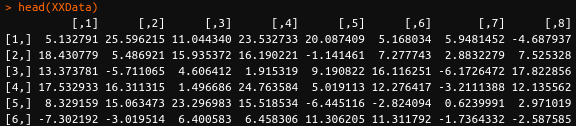
\includegraphics[scale=.75]{head.png}
\caption{Appel et résultat de la fonction head sur XXData}
\end{figure}
\noindent On observe qu'il y a 8 variables, lesquelles semblent etre quantitatives continues contenues dans l'intervalle $[-20;20]$.\\
La fonction $summary$ nous donne plus d'informations :
\begin{figure}[H]
\centering
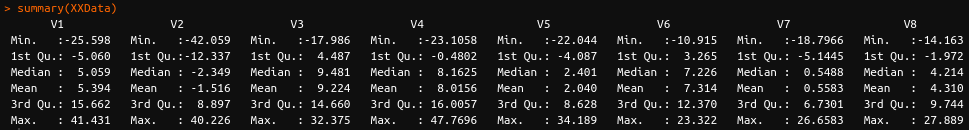
\includegraphics[scale=.5]{summary.png}
\caption{Appel et résultat de la fonction summary sur XXData}
\end{figure}
\noindent On observe que nos données sont contenues dans l'intervalles $[-50;50]$, avec des moyennes assez proches l'une de l'autre. Cet appel nous permet aussi de déterminer la médiane, les extremas, le premier et le troisième quartile de chacune de nos variables pour nos données.\\
\newpage
\noindent Observons ensuite le boxplot de nos données :
\begin{figure}[H]
\centering
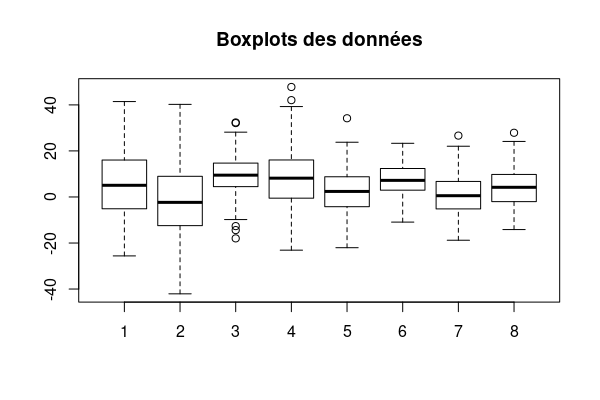
\includegraphics[scale=1]{boxplot.png}
\caption{Boxplot des variables de XXData obtenu via la fonction $boxplot$}
\end{figure}
\noindent On observe sur cette figure que, en effet, nos moyennes sont assez proches et que globalement les individus sont proches les uns des autres.\\
Pour finir, un dernier appel à la fonction $nrow$ nous indique qu'il y a 128 individus dans XXData.
\newpage
\section{ACP}
Le but de l'ACP (\emph{Analyse en composantes principales}) est de réduire le nombre de variables tout en conservant au maximum l'information.\\
Pour commencer, malgré que toutes nos données aient la même unité (pas d'unité) et le même intervalle de valeurs, nous allons les centrer et réduire :
\begin{figure}[H]
\centering
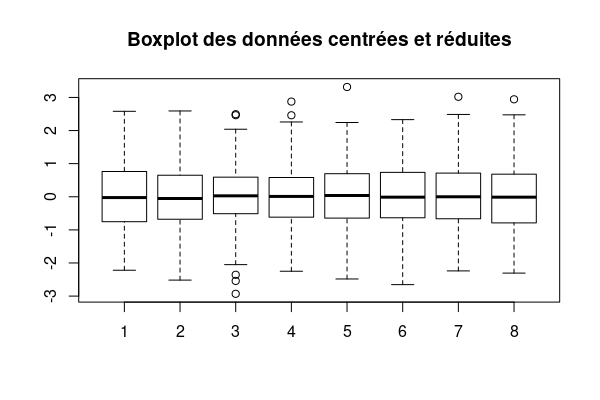
\includegraphics[scale=1]{boxplotCR.png}
\caption{Boxplots des données centrées et réduites.}
\end{figure}
\noindent Nous allons maintenant nous intéresser à la matrice de corrélation de nos variables. La diagonalisation de cette matrice nous permettra de définir le nombre de composantes à conserver.\begin{figure}[H]
\centering
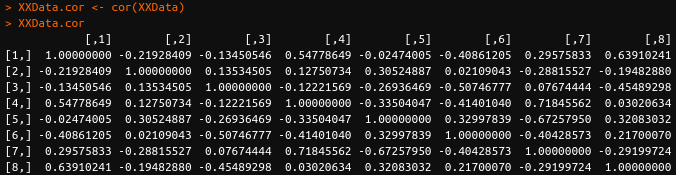
\includegraphics[scale=0.7]{cor.png}
\caption{Matrice de corrélation obtenue via la fonction $cor$}
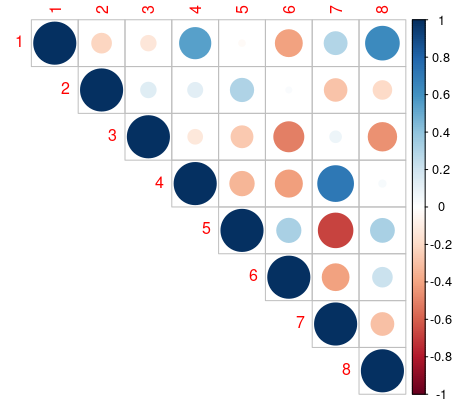
\includegraphics[scale=1]{corrplot.png}
\caption{Représentation de la matrice de corrélation générée via la fonction $corrplot$}
\end{figure}
\noindent On remarque une forte corrélation entre les variables $V5$-$V7$, $V4$-$V7$ et $V8$-$V1$, le reste des variables ne semblent pas fortement corrélées.\\
\newpage
\noindent Calculons maintenant les valeurs propres de cette matrice à l'aide de la fonction $eigen$ de R, nous obtenons :
\begin{figure}[H]
\centering
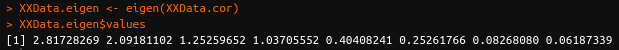
\includegraphics[scale=0.7]{eigen.png}
\caption{Valeurs propres de la matrice de corrélation}
\end{figure}
\noindent Selon le critère de Kaiser, nous devons conserver les 4 premières composantes car leur valeur propres sont $>1$.\\
Regardons le graphe en éboulis du pourcentage de la variance expliqué par composantes pour renforcer notre décision :
\begin{figure}[H]
\centering
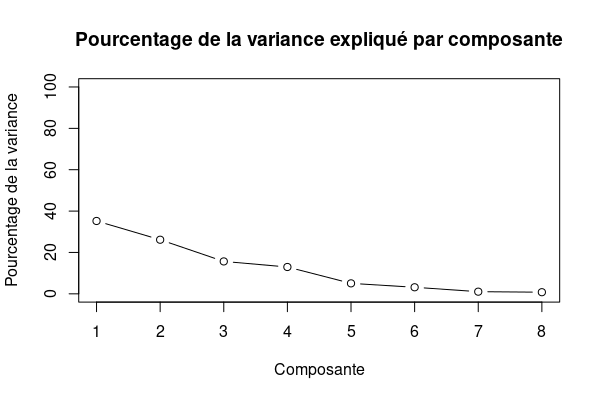
\includegraphics[scale=1]{coude.png}
\caption{Graphe en éboulis du pourcentage de variance expliqué par composante}
\end{figure}
\noindent Nous espérions observer un coude dans ce graphe, mais il n'y en a qu'un très léger après la 3e composante. Ce coude n'est pas assez satisfaisant que pour en déduire un nombre de composante à conserver. Nous décidons donc de conserver 4 composantes selon le critère de Kaiser, lesquelles nous permettrons d'expliquer $\approx 90\%$ de la variance totale comme nous l'indique la figure 9.
\begin{figure}[H]
\centering
\begin{tabular}{|c|c|}
\hline
Nombre de composantes & Variance expliquée cumulée (\%)\\
\hline
1&$35.21$\\
2&$61.36$\\
3&$77.02$\\
4&$89.98$\\
5&$95.03$\\
6&$98.19$\\
7&$99.22$\\
8&$100$\\
\hline
\end{tabular}
\caption{Pourcentages de la variance expliquée cumulés}
\end{figure}
\begin{figure}[H]
\centering
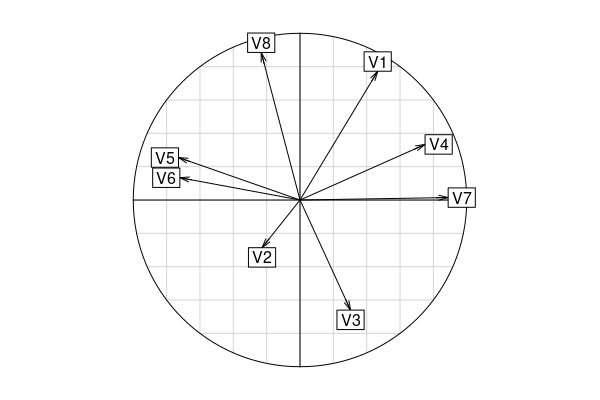
\includegraphics[scale=1]{corrcircle.png}
\caption{Cercle de corrélation généré via $corcirle$}
\end{figure}
\noindent Le cercle des corrélations corresponds à ce que nous avions observé dans la matrice de corrélations, $V5$ est opposé à $V7$ ce qui suggère une forte corrélation négative, $V1$ est proche de $V8$ et $V4$ est proche de $V7$ ce qui suggère une corrélation forte.
\begin{figure}[H]
\centering
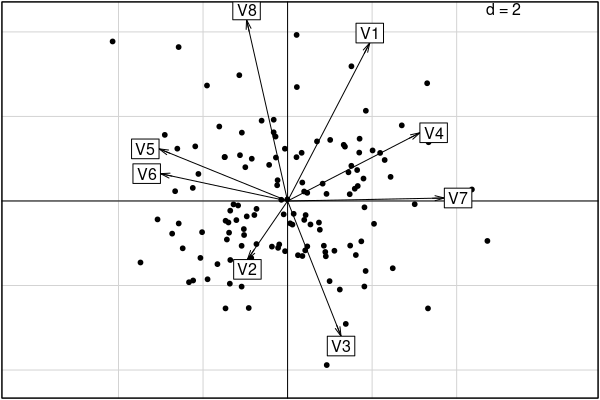
\includegraphics[scale=1]{scatter.png}
\caption{Scatterplot généré via la fonction $scatter$}
\end{figure}
Etant donné la dispersion des données sur le scatterplot, il est compliqué de tirer des conclusions.
\newpage
\section{Classification}
Pour tenter de classifier nos données, nous allons utiliser la méthode du \emph{k-means clustering}.
La première étape est de déterminer un nombre de cluster correct à utiliser. Pour ce faire nous allons étudier la variance intra groupe en fonction du nombre de cluster considérés, afin d'y localiser un coude ou une très nette diminution de la décroissance de la variance intra groupe.
\begin{figure}[H]
\centering
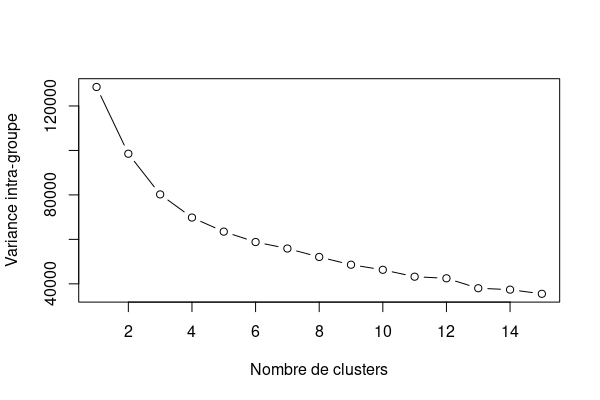
\includegraphics[scale=1]{nclust.png}
\caption{Variance intra groupe en fonction du nombre de cluster considéré}
\end{figure}
\noindent Il n'y a pas de net coude dans ce graphe, nous allons donc considérer 3 clusters car cela semble être le moment ou la diminution de la variance intra groupe devient plus faible.\\
La fonction $kmean$ appliquée sur nos composantes nous permet d'obtenir une classification.
\begin{figure}[H]
\centering
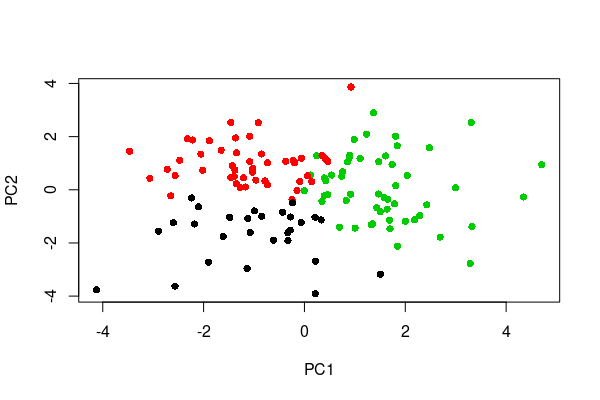
\includegraphics[scale=1]{class.png}
\caption{Classification obtenue avec la méthode $kmeans$ pour $k=3$}
\end{figure}
\subsection{Conclusion}
L'analyse en compsante principales nous a permis de réduire la dimension de nos données de 8 à 4 en conservant $\approx 90\% $ de l'information. Nous avons ensuite appliqué un algorithme de \emph{k-means clustering} afin de classifier nos données. Il est compliqué de discuter de la cohérence de cette classification étant donné l'aspect aléatoire et la similarité de nos variables dans le jeu de données originel. 
\newpage
\section{CLARA (Clustering LARge Applications}
% Finding Groups in Data An Intruction by Leonard Kaufman and Peter J. Rousseeuw.
Le \emph{clustering} (regroupement) d'un ensemble d'objets avec CLARA se fait en deux étapes. Premièrement, un échantillon est pioché aléatoirement dans l'ensemble des objets et regroupé en $k$ sous-ensembles en utilisant la méthode $k$-$medoid$, qui donne aussi $k$ objets représentatifs.\\
Ensuite, chaque objet n'appartenant pas a l'échantillon est affecté au plus proche des $k$ objets représentatifs. De cette façon, on obtient un clustering de l'ensemble des données. Une mesure de la qualité de ce clustering est obtenue en calculant la distance moyenne entre chaque objet de l'ensemble des données et de son objet représentatif. Apres avoir pioché aléatoirementf et regroupé 5 échantillons, celui qui a la plus petite distance moyenne est séléctionné.

\subsubsection{Méthode k-medoid en quelques mots}
L'algorithme $k-medoid$ est une approche de clustering utilisée pour partitionner un ensemble de données en $k$ groupes ou clusters. Dans cette méthode, chaque cluster est représenté par un seul point de donnée du cluster. Ce point est ce que l'on appelle le $medoid$.\\
Le terme medoid fait référence à un objet à l'intérieur du cluster pour lequel la dissimilitude moyenne entre ce point et tous les autres points du cluster est minimale. Il s'agit du point le plus au centre du cluster. Les medoids peuvent être considérés comme un exemple représentatif des membres de ce cluster.
Cette méthode est aussi appelée $PAM$ (Partioning Around Medoids).\\

\subsection{Description de l'algorithme}
Avec l'algorithme utilisé dans PAM, on séléctionne $k$ objets (les medoids) qui sont représentatifs ou localisés centralement, et les $k$ clusters sont construits autour de ces objets. L'effort principal de calcul qui sont fais dans l'algorithme  PAM est une recherche parmis un grand nombre de sous-ensembles de $k$ objets, pour un sous-ensemble produisant un regroupement satisfaisant et localement optimal. Si on augmente le nombre de données, la méthode k-medoid exacte est seulement faisable pour un nombre d'objets relativement petit car, dans le cas contraire, le temps de calcul devient énormement grand. L'allocation de la mémoire utilisée par PAM dépend principalement du nombre d'objets, qui est une fonction quadratique.\\

CLARA éffectue le clustering en conjonction avec la recherche par un ensemble d'objets représentatifs, qui devrait réprésenter un aspect différent de la structure de l'ensemble des données.\\
La méthode utilisée par CLARA est la sélection aléatoire de 5 (ou plus) échantillons d'objets. La taille des échantillons dépend du nombre de clusters. Pour un clustering en $k$ clusters, la taille de l'échantillon est donnée par $40+2k$. Le nombre de clusters doit varier entre 1 et 30, donc les échantillons contiennent entre 42 et 100 objets. Le choix d'utiliser une fonction du nombre de clusters pour la taille des échantillons est motivé par l'objectif d'avoir une probabilité raisonnable de trouver des objets de tous les échantillons "existants" dans au moins un des échantillons généré.\\
Pour la construction du premier échantillon, les objets sont séléctionnés par un nombre généré aléatoirement et ordonnés par un indice croissant. Chaque fois qu'un objet est pioché aléatoirement, on vérifie qu'il ne fait pas partie des objets déjà piochés. S'il n'avait pas encore été séléctionné, il est inséré à la bonne position dans le tableau.\\
Si la taille de l'échantillon est juste un petit peu plus petite que le nombre d'objets, il arrivera parfois que le même objet sera pioché  plusieurs fois de manière aléatoire. C'est pour cette raison qu'à chaque fois que le nombre d'objets est inférieur au double de la taille de l'échantillon, le générateur de nombres aléatoires est utilisé pour séléctionner les objets n'appartenants pas à l'échantillon. La construction d'autres échantillons est lancée en tenant compte des medoids qui ont été trouvés dans les échantillons précédents. A chaque étape de l'algorithme, le meilleur ensemble de medoids actuel est stocké dans un tableau. (Ce meilleur ensemble est celui pour lequel la distance moyenne pour l'ensemble des données est la plus petite trouvée jusqu'à présent). Un nouvel échantillon est construit en ajoutant des objets à ce meilleur ensemble, de la même manière que les objets ont été accumulés dans le premier échantillon.\\
Après le prélèvement d'un échantillon d'objets, celui-ci est divisé en $k$ groupes en utilisant le même algorithme que dans le programme PAM. Cet algorithme consiste en deux parties, appelées BUILD et SWAP. Dans BUILD, les objets représentatifs successifs sont séléctionnés dans le but d'obtenir la plus petite distance moyenne possible entre les objets (de l'échantillon) et leur object représentatif le plus similaire. Dans SWAP, on tente de diminuer la distance moyenne en remplacent les objets représentatifs.\\
Une fois que $k$ objets représentatifs ont été séléctionnés, chaque objets de l'ensemble de données (et pas seulement de l'échantillon) est attribué à l'objet représentatif le plus proche. La distance moyenne obtenue pour l'affectation est utilisée comme une mesure de la qualité du clustering. Une fois ce calcul effectué pour chacun des 5 échantillons, l'échantillon retenu est celui avec la plus petite distance moyenne possible.\\
Une analyse plus poussée est alors effectuée sur la dernière partition. La liste d'objets de chaque cluster est donnée, ainsi que le medoid et la taille du cluster (dans l'ensemble des données). Le programme va alors lister, pour chaque cluster, la distance moyenne et maximale pour son medoid. Aussi, la distance maximale est divisée par la distance minimal du medoid par rapport a un autre medoid. Cette valeur donne des informations sur l'étroitesse du cluster. Une petite valeur indique un cluster très serré, alors qu'une valeur qui dépasse 1 suggère un cluster faible.
\subsection{Exemple}
Tentons d'appliquer CLARA à notre jeu de données $XXData$. Pour ce faire nous allons utiliser la fonction $clara$ du package $cluster$ de R.
\begin{figure}[H]
\centering
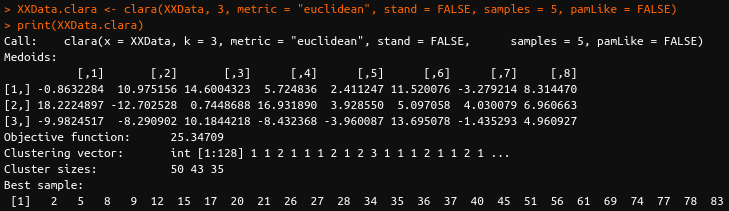
\includegraphics[scale=.65]{clara.png}
\caption{Résultat de l'application de la fonction $clara$ à notre jeu de données \emph{XXData}}
\end{figure}
\noindent Cette fonction retourne les informations suivantes :
\begin{itemize}
\item les \textbf{medoids}  : les médoids tels que définis plus haut.
\item \textbf{Clustering} : un vecteur indiquant à quel cluster apaprtient l'objet d'indice correspondant.
\item \textbf{sample} : Les individus contenus dans le meilleur échantillon, lequel sera utilisé par clara pour le partitionnement.
\end{itemize}
Et pour finir, le résultat de clara porté sur un graphique :
\begin{figure}[H]
\centering
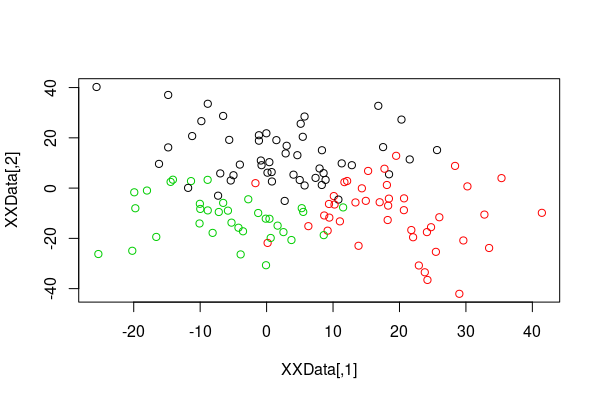
\includegraphics[scale=1]{claraclass.png}
\caption{Résultat graphique de Clara sur notre jeu de données XXData}
\end{figure}
\noindent A noter que pour cet exemple nous avons arbitrairement pris $k=3$ clusters, pour obtenir des résultats comparables à notre classification de la question 1.
\end{document}